\chapter{Analysing GDPR Compliance Requirements}
\label{chapter:information}

This chapter presents an analysis of information about activities associated with personal data and consent towards generating requirements for GDPR compliance. \autoref{sec:info:model} presents an analysis of GDPR in terms of stakeholders and interoperability of information between them along with an analysis of suitability of existing standards to represent it. Following this, \autoref{sec:info:compliance-questions} frames `compliance questions' that provide information requirements necessary to evaluate compliance. \autoref{sec:info:competency-questions} uses the compliance questions and identified gaps within the state of the art to formulate competency questions towards developing necessary ontologies for information representation of GDPR and activities involving personal data and consent. Finally, \autoref{sec:info:constraints} presents the assumptions and constraints over information that can be used to validate the information for correctness and completeness.

\section{Interoperability Model of Information based on GDPR}\label{sec:info:model}

This section presents an analyses of the GDPR in terms of information requirements of stakeholders and presents a model of interoperability between them. The model enables understanding the role of stakeholders in the compliance process and provides a framework to analyse approaches in the state of the art to meet requirements. The model also provides motivation to incorporate interoperability as a core requirement within representations of information towards GDPR compliance.
The work described in this section was published in a conference paper
\cite{} which was later expanded upon in a journal article \cite{}. % EURAS, IJSR

\subsection{Model of Information Interoperability}
The entity in terms of GDPR compliance are as follows: Data Subject (DS), Data Controller (DC), Data Processor (DP) and Supervisory Authority\footnote{Supervisory Authority are also referred to as Data Protection Commission or Regulatory Body} (SA). In addition to this, if a controller or processor uses a Data Management (DM) interface or service for their compliance operations, it can be a considered as a separate entity given its autonomous operations and possible provision by a third party. Though the GDPR does not mention or allude to the functionality of DM, it is included as a virtual entity in the analyses for practical reasons as a point of interoperability between entities.

With this, there are 11 possible points of interactions between entities, as summarised in Figure \ref{fig:info:interoperability-model}.
\begin{figure}[htbp]
    \centering
    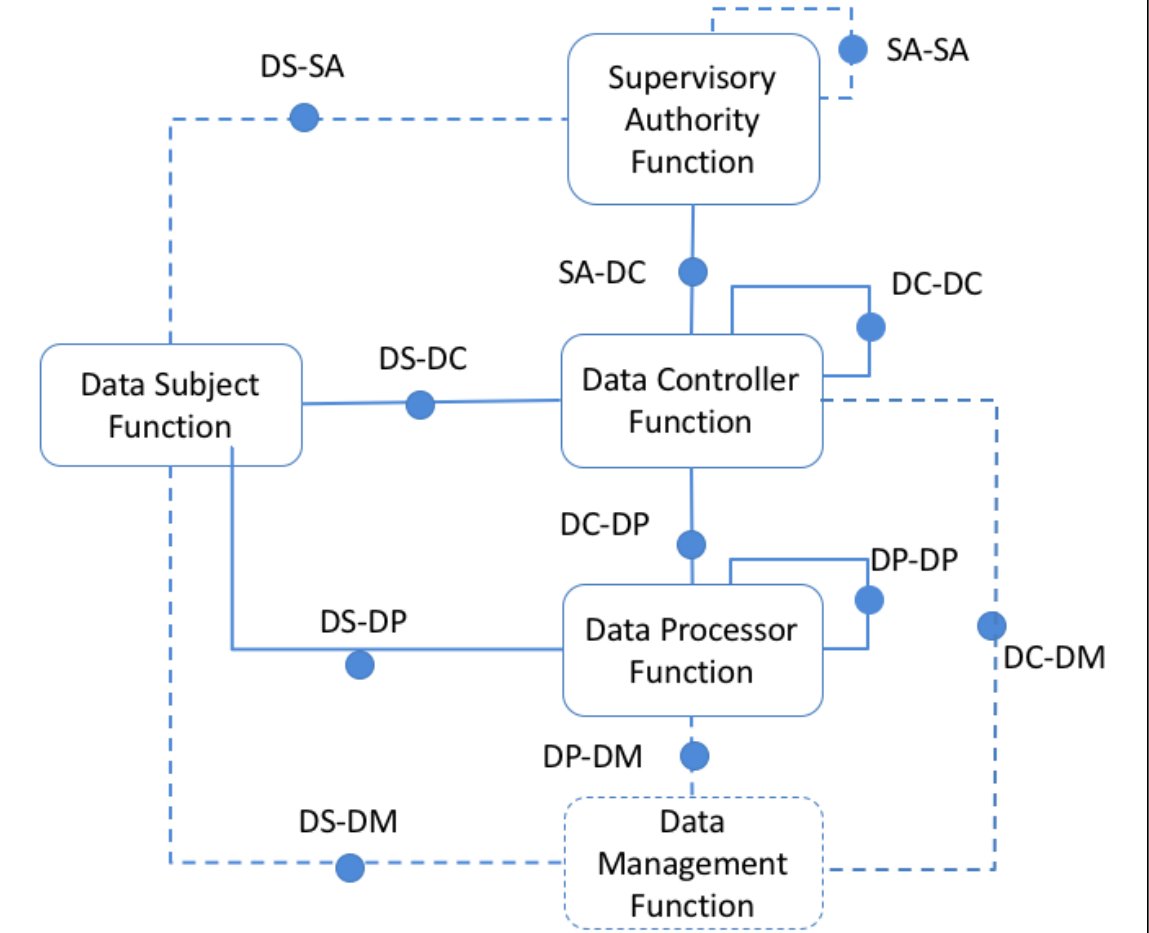
\includegraphics[width=0.75\linewidth]{img/interoperability-model.png}
    \caption{Model of information interoperability between entities based on requirements of GDPR \cite{x}}
    \label{fig:info:interoperability-model}
\end{figure}
These points of interactions consist of information exchange between entities, are are guided by the requirements of compliance. For example, the interaction between data subject and data controller consists of the data subject providing personal data to the controller, while the controller is required to provide a copy of provided personal data for fulfilment of rights granted by the GDPR.

Requirements gathered from GDPR guiding information flows between entities at points of interactions are categorised as follows:
\begin{itemize}
    \item Provenance records: GDPR requires controllers and processors to maintain provenance records of processing activities carried out under their responsibility in order to maintain and demonstrate compliance to supervisory authorities. Provenance records are also required to be maintained to enable provision of rights to the data subject, and for information sharing between controllers and third parties.
    \item Data sharing agreements: A controller and processor are required to have specific data sharing agreements in place that specify the processing activities to be carried out by the processor. 
    \item Consent information: Consent information regarding how it was provided to the data subject and the given consent are required to be recorded for demonstrating compliance as well as for providing the right to withdraw consent. Consent information is also required to be passed on to other controllers or third parties (at the request of the data subject) if processing involves more than one party.
    \item Compliance documentation: Processors are required to provide suitable guarantees to controllers regarding measures that ensure compliance with the GDPR. This information needs to be shared between controllers and processors, as well as demonstrated to supervisory authorities in the due process of evaluating compliance.
    \item Use of certifications: GDPR provides seals and certifications to be used to denote a certain degree of compliance based on existence of measures and processes that adhere to GDPR requirements. The presence of such seals and certifications as well as their associated information needs to be exchanged between entities to demonstrate trust and guarantees, such as between processors and controllers, or controllers and data subjects.
\end{itemize}

% opportunities for commonality and interoperability
% role of process flows, especially for processing activities regarding personal data and consent

\subsection{Suitability of existing standards}
% bodies: W3C, ISO, ISA2

% W3C standards for representing + state of the art analyses

\section{Compliance Questions}\label{sec:info:compliance-questions}

\section{Competency Questions}\label{sec:info:competency-questions}

\section{Constraints \& Assumptions for Validation}\label{sec:info:constraints}